
\section{Model Selection} \label{modsel}

\begin{table}[H]
\centering
\begin{tabular}{ |p{1.5cm}|p{8cm}|p{3cm}| }
    \hline
    Models: & Change from the best model: & $\Delta AIC$ from the best model \\
    \hline
    Mod1 &$-\beta_\text{HC} \ x_\text{HC,ij\text{k}} + \beta_\text{HC,\text{k}} \ x_\text{HC,ij\text{k}}$ & $0$ \\
    \hline
    Mod2 &$-\beta_\text{HC} \ x_\text{HC,ij\text{k}}$ & $3$ \\
    \hline
    Mod3 &$-\beta_{\text{C},\text{k}} \ x_\text{C,ij\text{k}} + \beta_{\text{C}} \ x_\text{C,ij\text{k}}$ & $958$ \\
    \hline
    Mod4 &$-\beta_{\text{H},\text{k}} \ x_\text{H,ij\text{k}} + \beta_{\text{H}} \ x_\text{H,ij\text{k}}$ & $14$ \\
    \hline
    Mod5 &$-\beta_{\text{C},\text{k}} \ x_\text{C,ij\text{k}} - \beta_\text{HC} \ x_\text{HC,ij\text{k}} + \beta_{\text{C}} \ x_\text{C,ij\text{k}}$ & $961$ \\
    \hline
    Mod6 &$-\beta_{\text{H},\text{k}} \ x_\text{H,ij\text{k}} - \beta_{\text{C},\text{k}} \ x_\text{C,ij\text{k}} + \beta_{\text{H}} \ x_\text{H,ij\text{k}} + \beta_{\text{C}} \ x_\text{C,ij\text{k}}$ & $972$ \\
    \hline
    Mod7 &$-\beta_{\text{H},\text{k}} \ x_\text{H,ij\text{k}} - \beta_\text{HC} \ x_\text{HC,ij\text{k}} + \beta_{\text{H}} \ x_\text{H,ij\text{k}}$ & $16$ \\
    \hline
    Mod8 &$-\beta_{\text{H},\text{k}} \ x_\text{H,ij\text{k}} - \beta_{\text{C},\text{k}} \ x_\text{C,ij\text{k}} - \beta_\text{HC} \ x_\text{HC,ij\text{k}} + \beta_{\text{H}} \ x_\text{H,ij\text{k}} + \beta_{\text{C}} \ x_\text{C,ij\text{k}}$ & $974$ \\
    \hline
\end{tabular}
\caption{Change in AIC from the best model}
\label{table:AICchangeCovid}
\end{table}

\noindent The best model can be seen in Equation \ref{eq:bestmodelcovid}, but below I will show some neighboring models to the best one that I compared it to in Table \ref{table:AICchangeCovid} along with the difference between the AIC for the best model and these neighboring models. In model $1$, the interaction between the home court advantage and covid is replaced with a three way interaction between home court advantage, covid and each scoring type. In model $2$, the interaction between the home court advantage and covid is removed. In model $3$, the interaction between covid and each scoring type is replaced with a single covid term. In model $4$, the interaction between home court advantage and each scoring type is replaced with a single home court term. Model 5 is almost the same as model 3 but the interaction between home court and covid is removed. Model 6 has both the interaction between home court and scoring type and the interaction between covid and scoring type replaced with just one term for home court and one term for covid. Model 7 is similar to model 4, but the interaction between home court and covid is removed. Finally, model 8 is the same as model 6 but the interaction between home court and covid is removed.

\section{Best Model} \label{bestmod}

\noindent After a great deal of testing, I have found that the best model to use for this data is,

\begin{equation}
    \log(\lambda_{i,j,\text{k}}) = \beta_\text{k} + \beta_{\text{H},\text{k}} \ x_\text{H,ij\text{k}} + \beta_{\text{C},\text{k}} \ x_\text{C,ij\text{k}} + \beta_\text{HC} \ x_\text{HC,ij\text{k}} + \gamma_{\text{A},i,\text{k}} + \gamma_{\text{D},j,\text{k}}.
\label{eq:bestmodelcovid}
\end{equation}

\noindent The scoring type is denoted by index $\text{k} = 1,2,3$, the attacking team is denoted by index $i$, and the defending team is denoted by index $j$. $x_\text{H,ij\text{k}}$, $x_\text{C,ij\text{k}}$, and $x_\text{HC,ij\text{k}}$ are dummy, or indicator, variables. They indicate if we have a match where attacking team $i$ has home court advantage, if we have a match played during the Covid-season, or if we have a match with home court advantage during the Covid-season, respectively. Table \ref{table:fixedEffCovid} shows the fixed effects of the model in Equation \ref{eq:bestmodelcovid} together with their standard deviations, and Table \ref{table:fixedEffExpCovid} shows the percent the expected number of scores changes for each type when the different estimated values are included. This model is very similar to the one used in \cite{fotballglmm}, but I have added a covid term and an interaction between home court and covid, and since there are three ways of scoring in basketball, i have added an interaction between each scoring types and home court term and the covid term.

The random effects in the model are $\gamma_{\text{A},i,\text{k}}$ and $\gamma_{\text{D},j,\text{k}}$. They are independent and identically distributed, with $\gamma_{\text{A},i,\text{k}} \sim N(0,\tau_{\text{A},\text{k}}^2)$ and $\gamma_{\text{D},i,\text{k}} \sim N(0,\tau_{\text{D},\text{k}}^2)$. These variances can be seen in Table \ref{table:randomEffCovidVar}. We assume that attack strength and defence strength of team $i$ are independent of one another, i.e. $\gamma_{\text{A},i,\text{k}}$ and $\gamma_{\text{D},i,\text{k}}$ are independent for each scoring type, but I will discuss this assumption in Section \ref{corr_covid}. These random effects together with the fixed effects gives the conditional expected number of scores from scoring type $\text{k}$ that attacking team $i$ will score against defending team $j$ by the equation,

\begin{equation}
    E\big[y_{i,j,\text{k}} | \gamma_{\text{A},i,\text{k}}, \gamma_{\text{D},j,\text{k}}\big] = \text{exp}\big\{ \beta_\text{k} + \beta_{\text{H},\text{k}} \ x_\text{H,ij\text{k}} + \beta_{\text{C},\text{k}} \ x_\text{C,ij\text{k}} + \beta_\text{HC} \ x_\text{HC,ij\text{k}} + \gamma_{\text{A},i,\text{k}} + \gamma_{\text{D},j,\text{k}} \big\}.
\end{equation}

\begin{table}[!ht]
\centering
\begin{tabular}{ |p{.3cm}|p{3cm}|p{3cm}|p{3cm}|p{3cm}|  }
    \hline
    $\text{k}$ & $\hat\beta_\text{k} \pm SD(\hat\beta_\text{k})$& $\hat\beta_{\text{H},\text{k}} \pm SD(\hat\beta_{\text{H},\text{k}})$ & $\hat\beta_{\text{C},\text{k}} \pm SD(\hat\beta_{\text{C},\text{k}})$ & $\hat\beta_\text{HC} \pm SD(\hat\beta_\text{HC})$ \\
    \hline
    $1$ & $2.8412 \pm 0.0118$ & $0.0343 \pm 0.0035$ & $-0.0229 \pm 0.0063$ & $-0.0124 \pm 0.0060$ \\
    $2$ & $3.3695 \pm 0.0099$ & $0.0166 \pm 0.0027$ & $-0.0226 \pm 0.0052$ & $-0.0124 \pm 0.0060$ \\
    $3$ & $2.3207 \pm 0.0186$ & $0.0277 \pm 0.0045$ & $+0.2079 \pm 0.0072$ & $-0.0124 \pm 0.0060$ \\
    \hline
\end{tabular}
\caption{Fixed Effects $\pm$ Standard Deviations}
\label{table:fixedEffCovid}
\end{table}

\begin{table}[!ht]
\centering
\begin{tabular}{ |p{.5cm}|p{2cm}|p{2cm}|p{2cm}|p{2cm}|  }
    \hline
    $\text{k}$ & $e^{\hat\beta_\text{k}}$ & $e^{\hat\beta_{\text{H},\text{k}}}$ & $e^{\hat\beta_{\text{C},\text{k}}}$ & $e^{\hat\beta_\text{HC}}$ \\
    \hline
    $1$ & $\approx 17$ & $\approx 3.49\%$ & $\approx -2.26\%$ & $\approx -1.23\%$ \\
    $2$ & $\approx 29$ & $\approx 1.68\%$ & $\approx -2.23\%$ & $\approx -1.23\%$ \\
    $3$ & $\approx 10$ & $\approx 2.81\%$ & $\approx +23\%$ & $\approx -1.23\%$ \\
    \hline
\end{tabular}
\caption{Exponential value of the Fixed Effects}
\label{table:fixedEffExpCovid}
\end{table}

\section{Correlation between attack and defence strength} \label{corr_covid}

\begin{figure}[H]
    \centering
    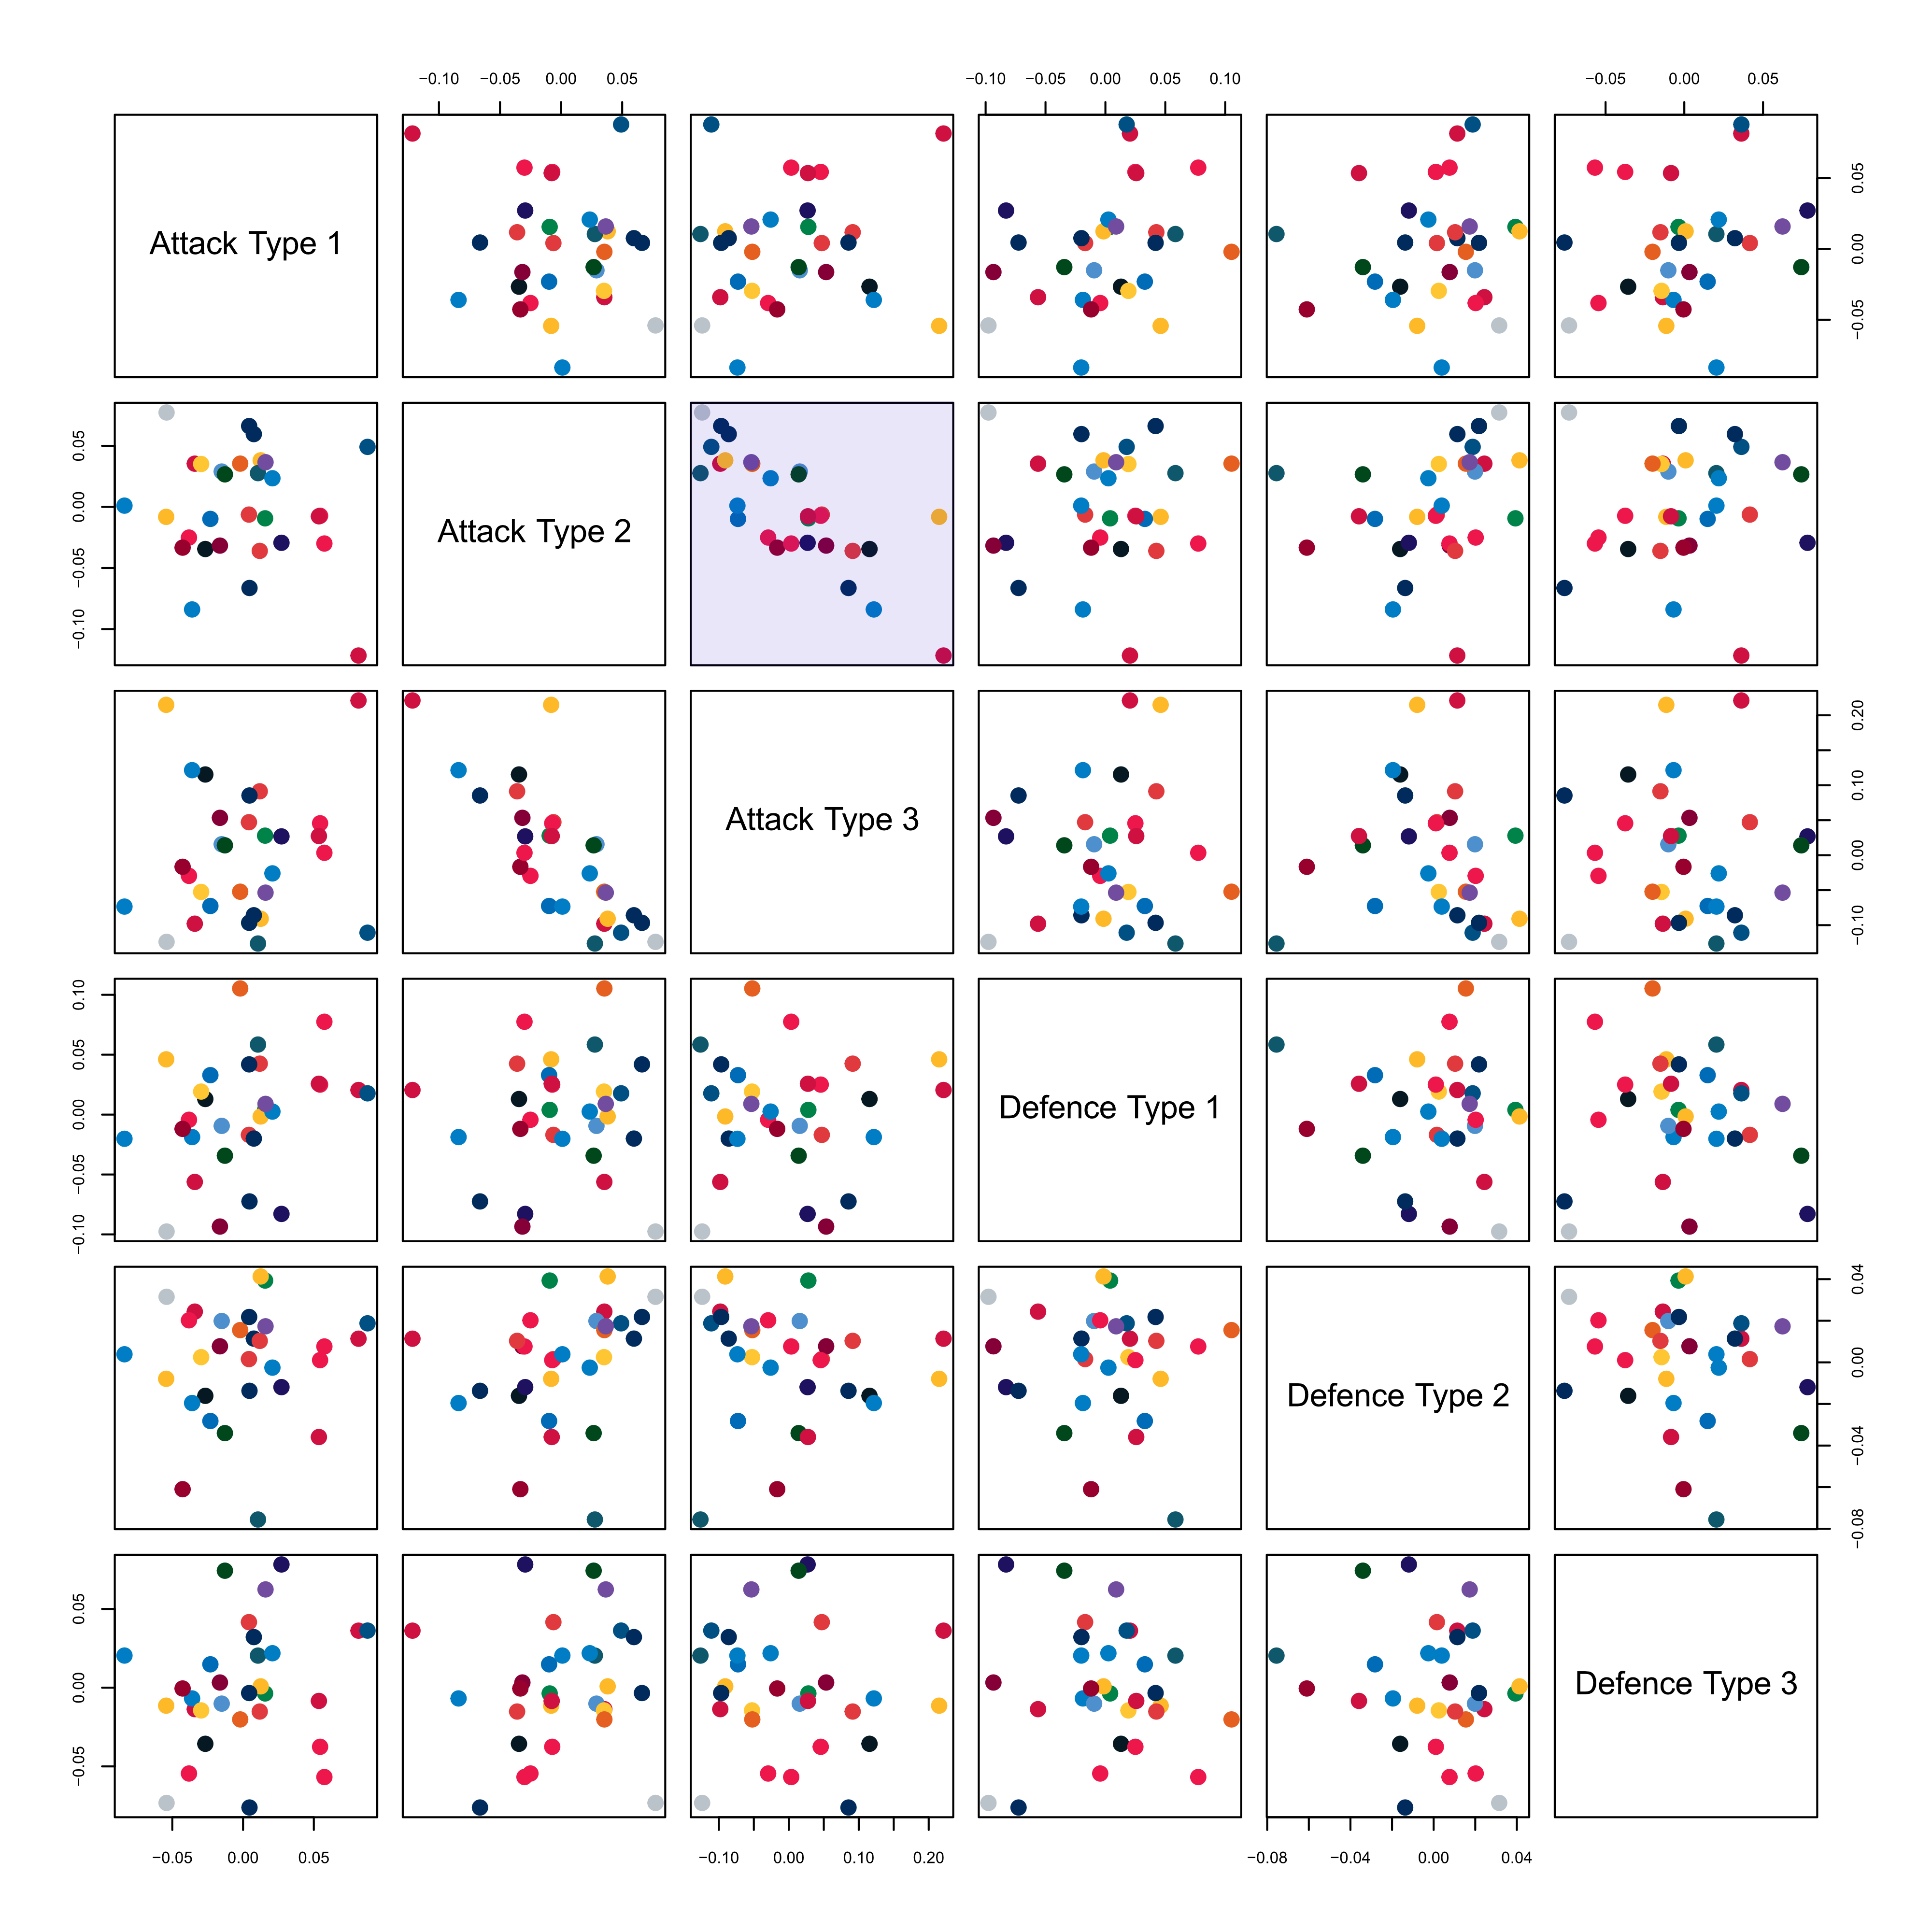
\includegraphics[width=1\textwidth]{Figures/Corr.png}
    \caption[Correlation]{Correlation between the different attacking and defending strengths}
    \label{fig:Corr}
\end{figure}

\noindent The correlation between attacking and defending strength for each scoring type can be seen in Figure \ref{fig:Corr}. From this figure we can see that there is a negative correlation between attacking strength of type 2 and 3 in the cell in row 2, column 3. This entails that teams who are very good at scoring with type 3 are bad at scoring or unwilling to score with type 2, and vice versa. The only team not following this norm is the Golden State Warriors, GSW. This makes sense because they have won 4 of the last 8 seasons excluding the 2019-2020 season, which means that they have been consistently good during these 8 seasons. There doesn't seem to be any correlation between attack and defence strengths, so the assumption that attack strength and defence strength are independent seem to mostly hold up looking at the correlation table.

\section{Strength of each team}

\noindent The attacking strengths for each team can be seen in Figure \ref{fig:Attack1}, \ref{fig:Attack2}, and \ref{fig:Attack3}, and the defending strengths can be seen in Figure \ref{fig:Defence1}, \ref{fig:Defence2}, and \ref{fig:Defence3}. Here we see which teams are the strongest at each scoring type. The expected values of the strength parameters are zero, so when a team has a strength of $0.10$, it is $e^{0.10} \approx 11\%$ stronger that the mean strength. This means that they will score $11\%$ more scores than a team with average strength. \\

\begin{table}[H]
\centering
\begin{tabular}{ |p{.5cm}|p{2cm}|p{2cm}|  }
    \hline
    $\text{k}$ & $\tau_{\text{A},\text{k}}^2$ & $\tau_{\text{D},\text{k}}^2$ \\
    \hline
    $1$ & $0.0016857$ & $0.0023295$ \\
    $2$ & $0.0020435$ & $0.0007715$ \\
    $3$ & $0.0084381$ & $0.0016362$ \\
    \hline
\end{tabular}
\caption{Variances of the Random Effects}
\label{table:randomEffCovidVar}
\end{table}

\noindent The variances for the random effects can be seen in Table \ref{table:randomEffCovidVar}. From this table we can see that the three points attacking strength vary much more than the other attacking types and all defending types. This makes sense because the three point shot is the hardest scoring type, so all teams cannot be equally as good with that type. Also the two-pointers don't vary as much, which means that all teams score almost the same amount of two-pointers.

\begin{figure}[H]
    \centering
    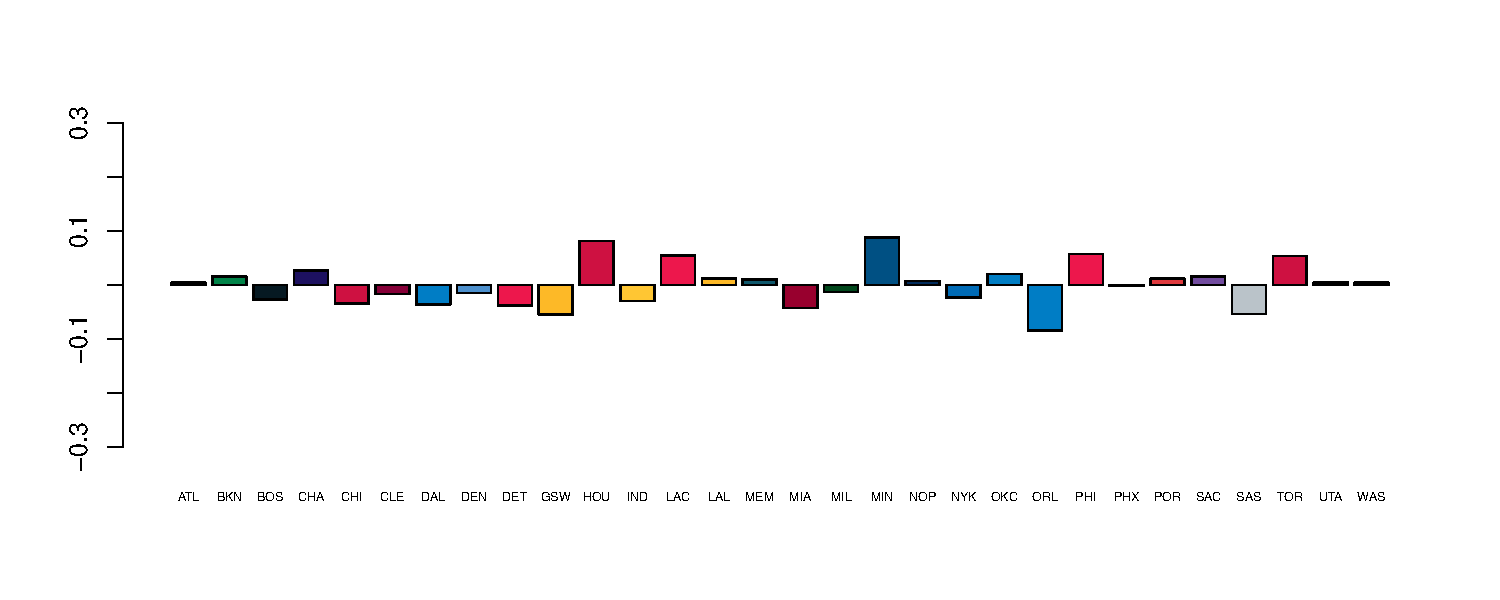
\includegraphics[width=1\textwidth]{Figures/Attack1.pdf}
    \caption[Attack1]{Strength of attacking type 1.}
    \label{fig:Attack1}
\end{figure}

\begin{figure}[H]
    \centering
    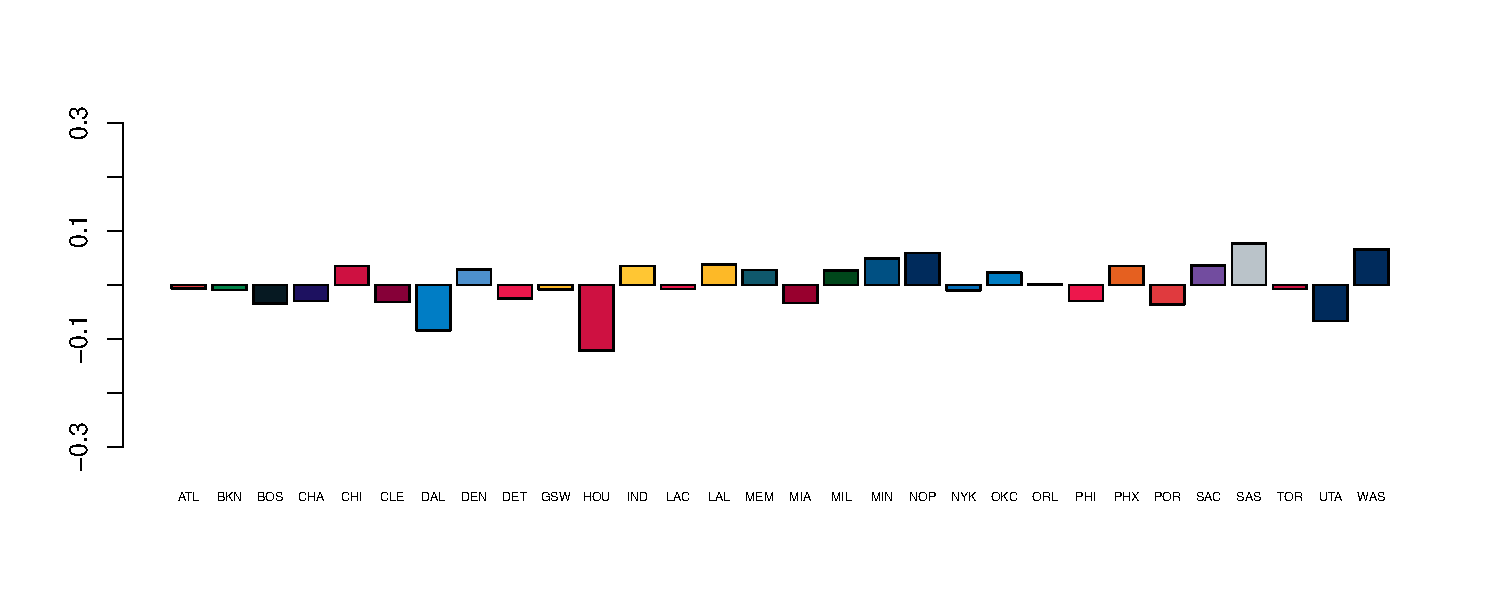
\includegraphics[width=1\textwidth]{Figures/Attack2.pdf}
    \caption[Attack2]{Strength of attacking type 2.}
    \label{fig:Attack2}
\end{figure}


\begin{figure}[H]
    \centering
    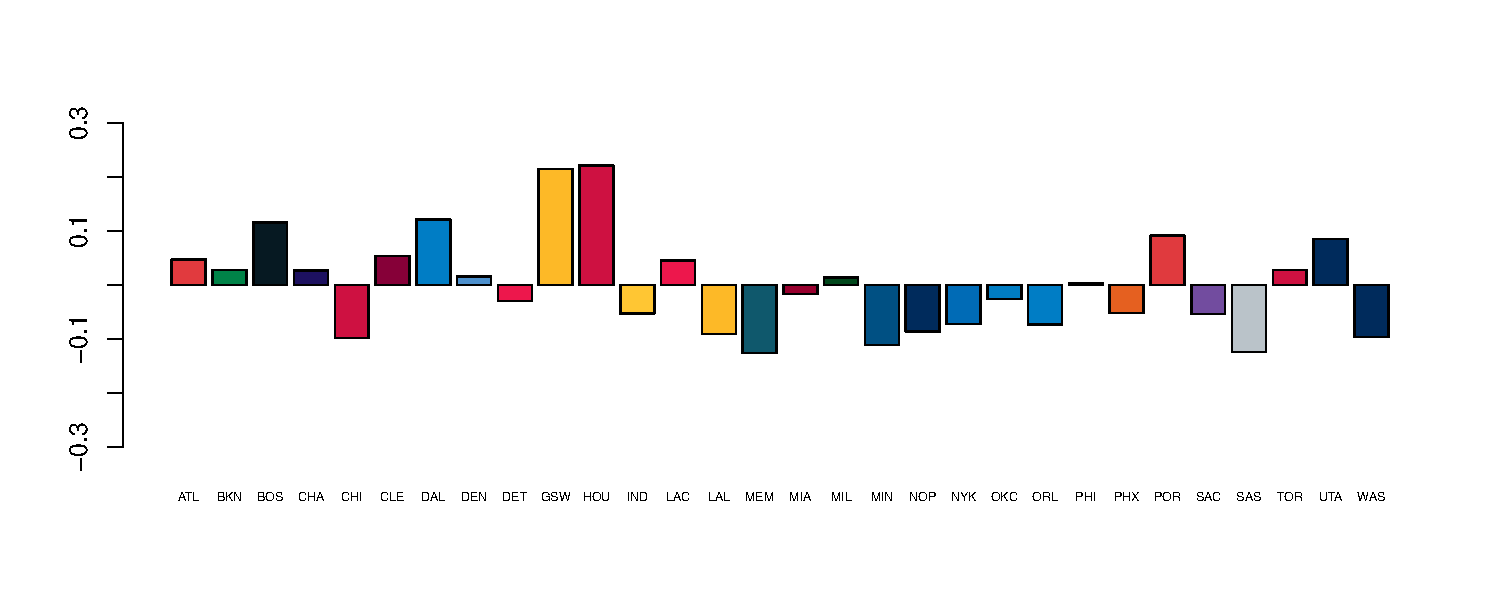
\includegraphics[width=1\textwidth]{Figures/Attack3.pdf}
    \caption[Attack3]{Strength of attacking type 3.}
    \label{fig:Attack3}
\end{figure}

\begin{figure}[H]
    \centering
    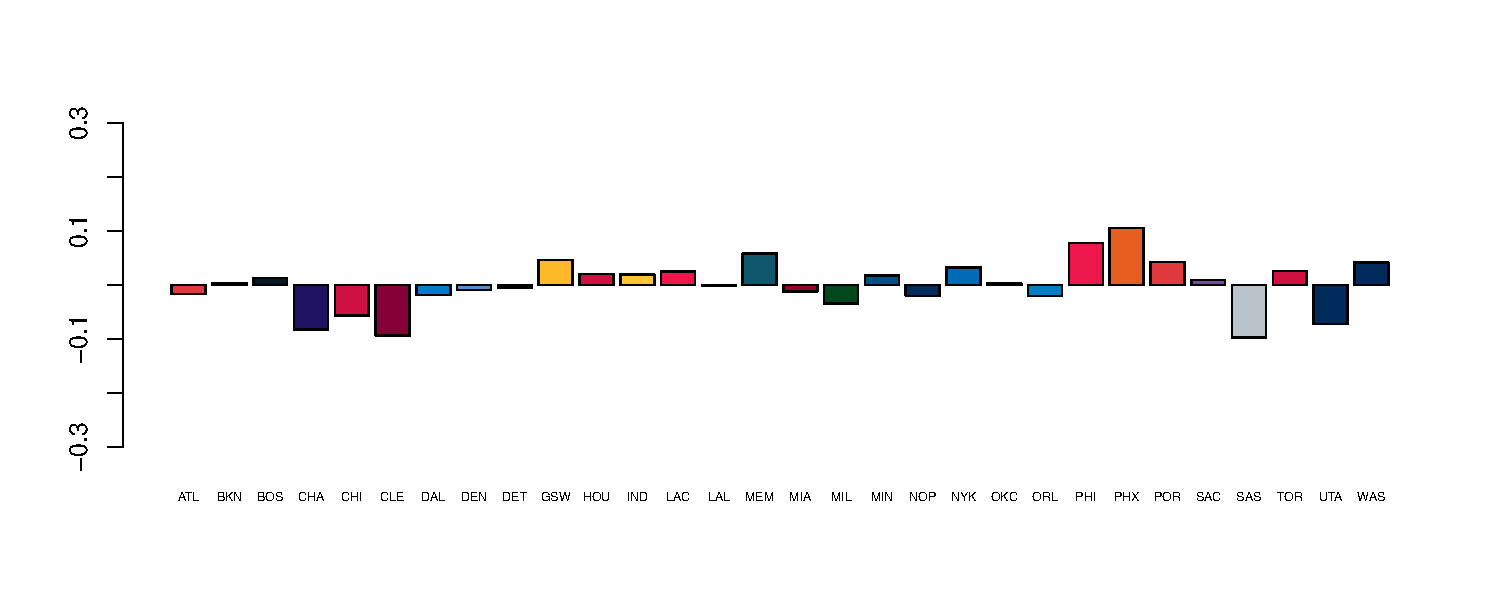
\includegraphics[width=1\textwidth]{Figures/Defence1.pdf}
    \caption[Attack1]{Strength of defending type 1.}
    \label{fig:Defence1}
\end{figure}

\begin{figure}[H]
    \centering
    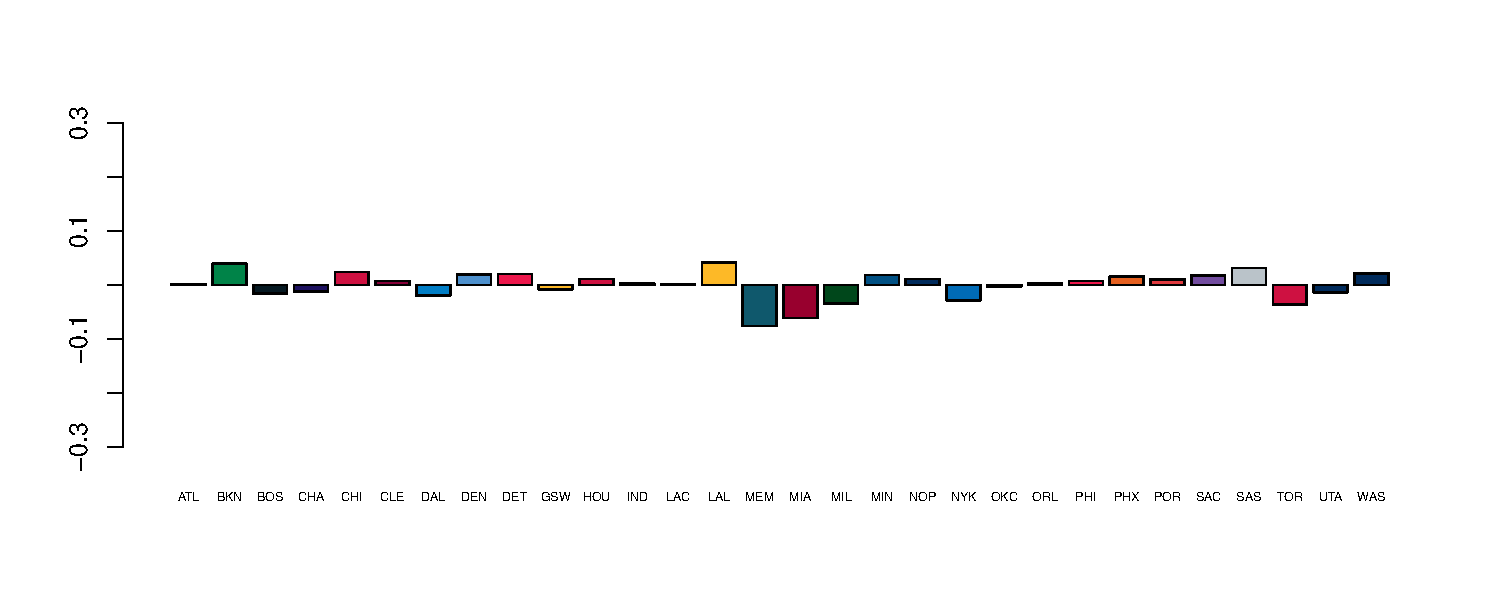
\includegraphics[width=1\textwidth]{Figures/Defence2.pdf}
    \caption[Attack2]{Strength of defending type 2.}
    \label{fig:Defence2}
\end{figure}

\begin{figure}[H]
    \centering
    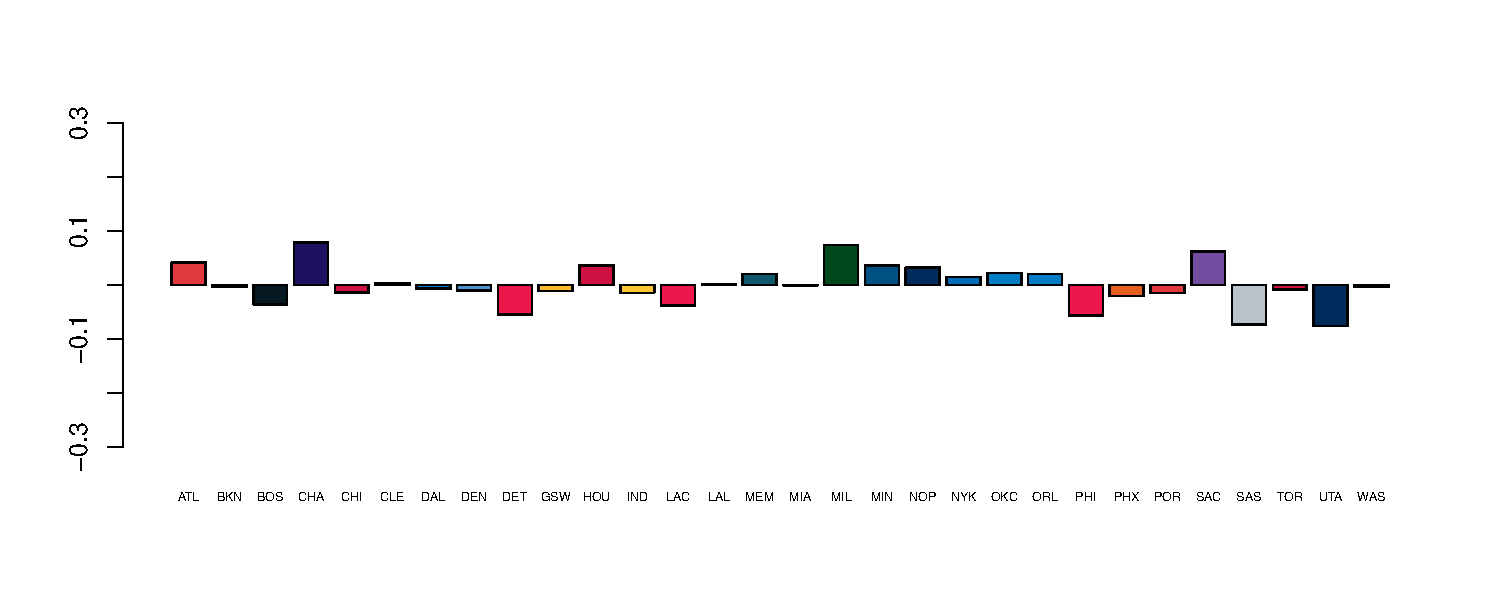
\includegraphics[width=1\textwidth]{Figures/Defence3.pdf}
    \caption[Attack3]{Strength of defending type 3.}
    \label{fig:Defence3}
\end{figure}

\section{Covid-19 impact and home court advantage}

\noindent From Table \ref{table:fixedEffExpCovid} we can see the influence that the home court had and that Covid had on every scoring type. In the last column, we can also see that during covid, the homecourt advantage got $1.23\%$ smaller during covid. There could be many reasons why the homecourt advantage got smaller, but one explanation of this could be that there were no fans spectating, and with less fans the home team didn't get the same boost that a full arena would give them. \\

\section{Number of fans}

\noindent Another interesting influence on the number of scores could be the number of fans spectating. The best model for this is,

\begin{equation}
\begin{aligned}
    \log(\lambda_{i,j,\text{k}}) &= \beta_\text{k} + \beta_{\text{H},\text{k}} \ x_\text{H,ij\text{k}} + \beta_{\text{FANS},\text{k}} \ x_\text{FANS,ij\text{k}} \\
    &+ \beta_\text{H.FANS} \ x_\text{H.FANS,ij\text{k}} + \gamma_{\text{A},i,\text{k}} + \gamma_{\text{D},j,\text{k}},
\label{eq:bestmodelfans}
\end{aligned}
\end{equation}

\noindent which I found using the same method for testing as in Section \ref{modsel}. This model is almost identical to the model in Equation \ref{eq:bestmodelcovid} but instead of Covid we are using the number of fans present at a match. $x_\text{FANS}$ and $x_\text{H.FANS}$ is then the number of fans present in a normal match and a normal match at home respectively. When the number of fans at a match is zero, this model is essentially the same as the model in Equation \ref{eq:bestmodelcovid} during covid. Table \ref{table:fixedEffExpFans} show the influence that a single fan has and the influence $20.000$ fans has on the total amount of scores of each type. The last column show the influence added when having home court advantage. This table also show the amount of points during covid, because there were no fans present. It suggest that when the number of fans increased, the total amount of one-pointers and two-pointers increased but the total amount of three-pointers decreased. This is because during covid, the total amount of three-pointers scored in a match increased, as shown in Table \ref{table:fixedEffExpCovid}.

\begin{table}[!ht]
\centering
\begin{tabular}{ |p{.5cm}|p{2cm}|p{3cm}|p{2cm}|p{2cm}| }
    \hline
    $\text{k}$ & $e^{\hat\beta_\text{k}}$ & $e^{\hat\beta_{\text{FANS},\text{k}}}$ & $e^{\hat\beta_{\text{FANS},\text{k}} \cdot 20000}$ & $\beta_\text{H.FANS}$ \\
    \hline
    $1$ & $\approx 17$ & $\approx 0.0001\%$ & $\approx 2.1\%$ & $\approx 0.0001\%$ \\
    $2$ & $\approx 28$ & $\approx 0.0001\%$ & $\approx 2.5\%$ & $\approx 0.0001\%$ \\
    $3$ & $\approx 13$ & $\approx -0.0012\%$ & $\approx -20.7\%$ & $\approx 0.0001\%$ \\
    \hline
\end{tabular}
\caption{Exponential value of the Fixed Effects using the model with fans}
\label{table:fixedEffExpFans}
\end{table}

\newpage

\section{Extension of the best model}

\noindent This thesis has only used the strength of a team according to 8 seasons worth of data, but because some teams change a lot inbetween and during seasons, a more interesting approach could be to use the AR(1) process to find the strengths of each team where they changes during the seasons. This could tell us if some teams tend to be stronger at the start, middle or end of a season, and how their strengths have changed throughout the years. But since there are some breaks in a season, one could maybe use the OU process to find the strengths during a season. The OU process can account for irregularities of the times where values are recorded, and can therefore be more useful. This new OU model has the same formula as the best model in section \ref{bestmod}, but the random effects are now modelled as a OU process. Tables \ref{table:fixedEffCovidOU} and \ref{table:fixedEffExpCovidOU} show the fixed effects and the exponential of the fixed effects respectively. These tables are pretty similar to tables \ref{table:fixedEffCovid} and \ref{table:fixedEffExpCovid}, but the covid term now give a positive impact on one- and two-poiners. This may be because now the attacking strengths of each team are not constant, but changes over time, so their strengths during covid could be slightly lower to account for this. This can be seen in Figures \ref{fig:OU1}, \ref{fig:OU2}, and \ref{fig:OU3} where the highlighted areas are the covid season. From Figure \ref{fig:OU3} we can see that the attacking strengths have increased a lot throughout the years for every team. Figures \ref{fig:GSW_2_OU}, \ref{fig:GSW_3_OU}, \ref{fig:HOU_2_OU}, and \ref{fig:HOU_3_OU} show the attacking strengths of the Golden State Warriors and Houston Rockets for both two-pointers and three-pointers. These two teams had the best three-points strengths, so it will be interesting to see how they compare throughout the years. We see that GSW has been very consistent with their strengths except for their two-pointer strength in the later seasons, but HOU have been very bad with two-pointers and inconsistent with three-pointers. This is due to them losing the players who scored three-pointers for them and GSW has kept most of theirs.

\begin{table}[!ht]
\centering
\begin{tabular}{ |p{.3cm}|p{3cm}|p{3cm}|p{3cm}|p{3cm}|  }
    \hline
    $\text{k}$ & $\hat\beta_\text{k} \pm SD(\hat\beta_\text{k})$& $\hat\beta_{\text{H},\text{k}} \pm SD(\hat\beta_{\text{H},\text{k}})$ & $\hat\beta_{\text{C},\text{k}} \pm SD(\hat\beta_{\text{C},\text{k}})$ & $\hat\beta_\text{HC} \pm SD(\hat\beta_\text{HC})$ \\
    \hline
    $1$ & $2.8298 \pm 0.0148$ & $0.0339 \pm 0.0035$ & $0.0387 \pm 0.0230$ & $-0.0126 \pm 0.0061$ \\
    $2$ & $3.3645 \pm 0.0147$ & $0.0167 \pm 0.0028$ & $0.0158 \pm 0.0224$ & $-0.0126 \pm 0.0061$ \\
    $3$ & $2.3134 \pm 0.0150$ & $0.0278 \pm 0.0045$ & $0.0926 \pm 0.0240$ & $-0.0126 \pm 0.0061$ \\
    \hline
\end{tabular}
\caption{Fixed Effects $\pm$ Standard Deviations for the OU model}
\label{table:fixedEffCovidOU}
\end{table}

\begin{table}[!ht]
\centering
\begin{tabular}{ |p{.5cm}|p{2cm}|p{2cm}|p{2cm}|p{2cm}|  }
    \hline
    $\text{k}$ & $e^{\hat\beta_\text{k}}$ & $e^{\hat\beta_{\text{H},\text{k}}}$ & $e^{\hat\beta_{\text{C},\text{k}}}$ & $e^{\hat\beta_\text{HC}}$ \\
    \hline
    $1$ & $\approx 17$ & $\approx 3.45\%$ & $\approx 3.95\%$ & $\approx -1.25\%$ \\
    $2$ & $\approx 29$ & $\approx 1.68\%$ & $\approx 1.59\%$ & $\approx -1.25\%$ \\
    $3$ & $\approx 10$ & $\approx 2.81\%$ & $\approx 9.70\%$ & $\approx -1.25\%$ \\
    \hline
\end{tabular}
\caption{Exponential value of the Fixed Effects for the OU model}
\label{table:fixedEffExpCovidOU}
\end{table}

\begin{figure}[H]
    \centering
    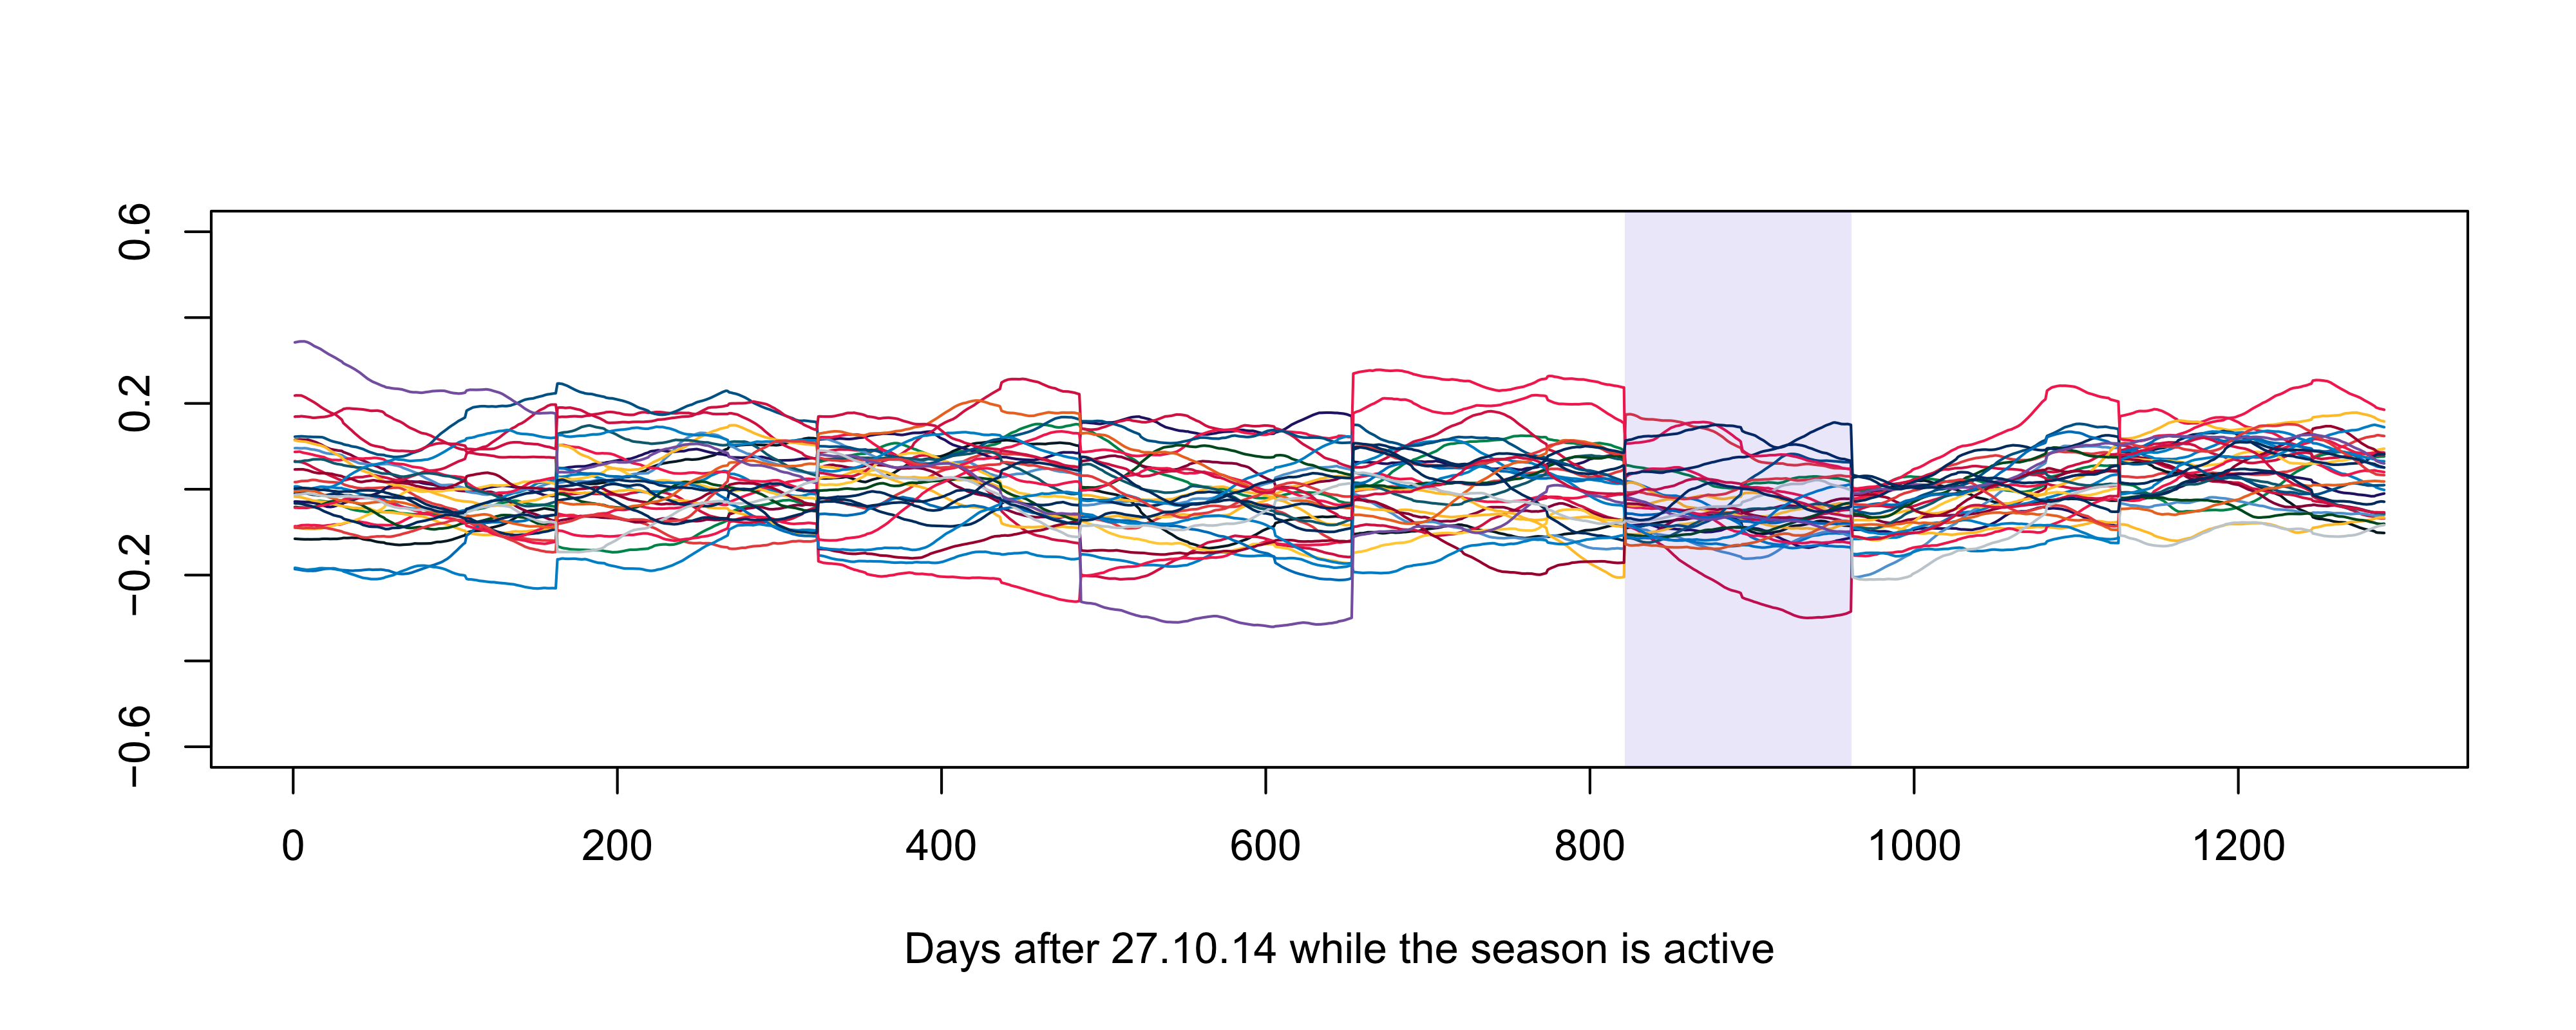
\includegraphics[width=1\textwidth]{Figures/OU1.png}
    \caption[OU1]{Strength of attacking type 1 using the OU model where the highlighted area is the covid season}
    \label{fig:OU1}
\end{figure}

\begin{figure}[H]
    \centering
    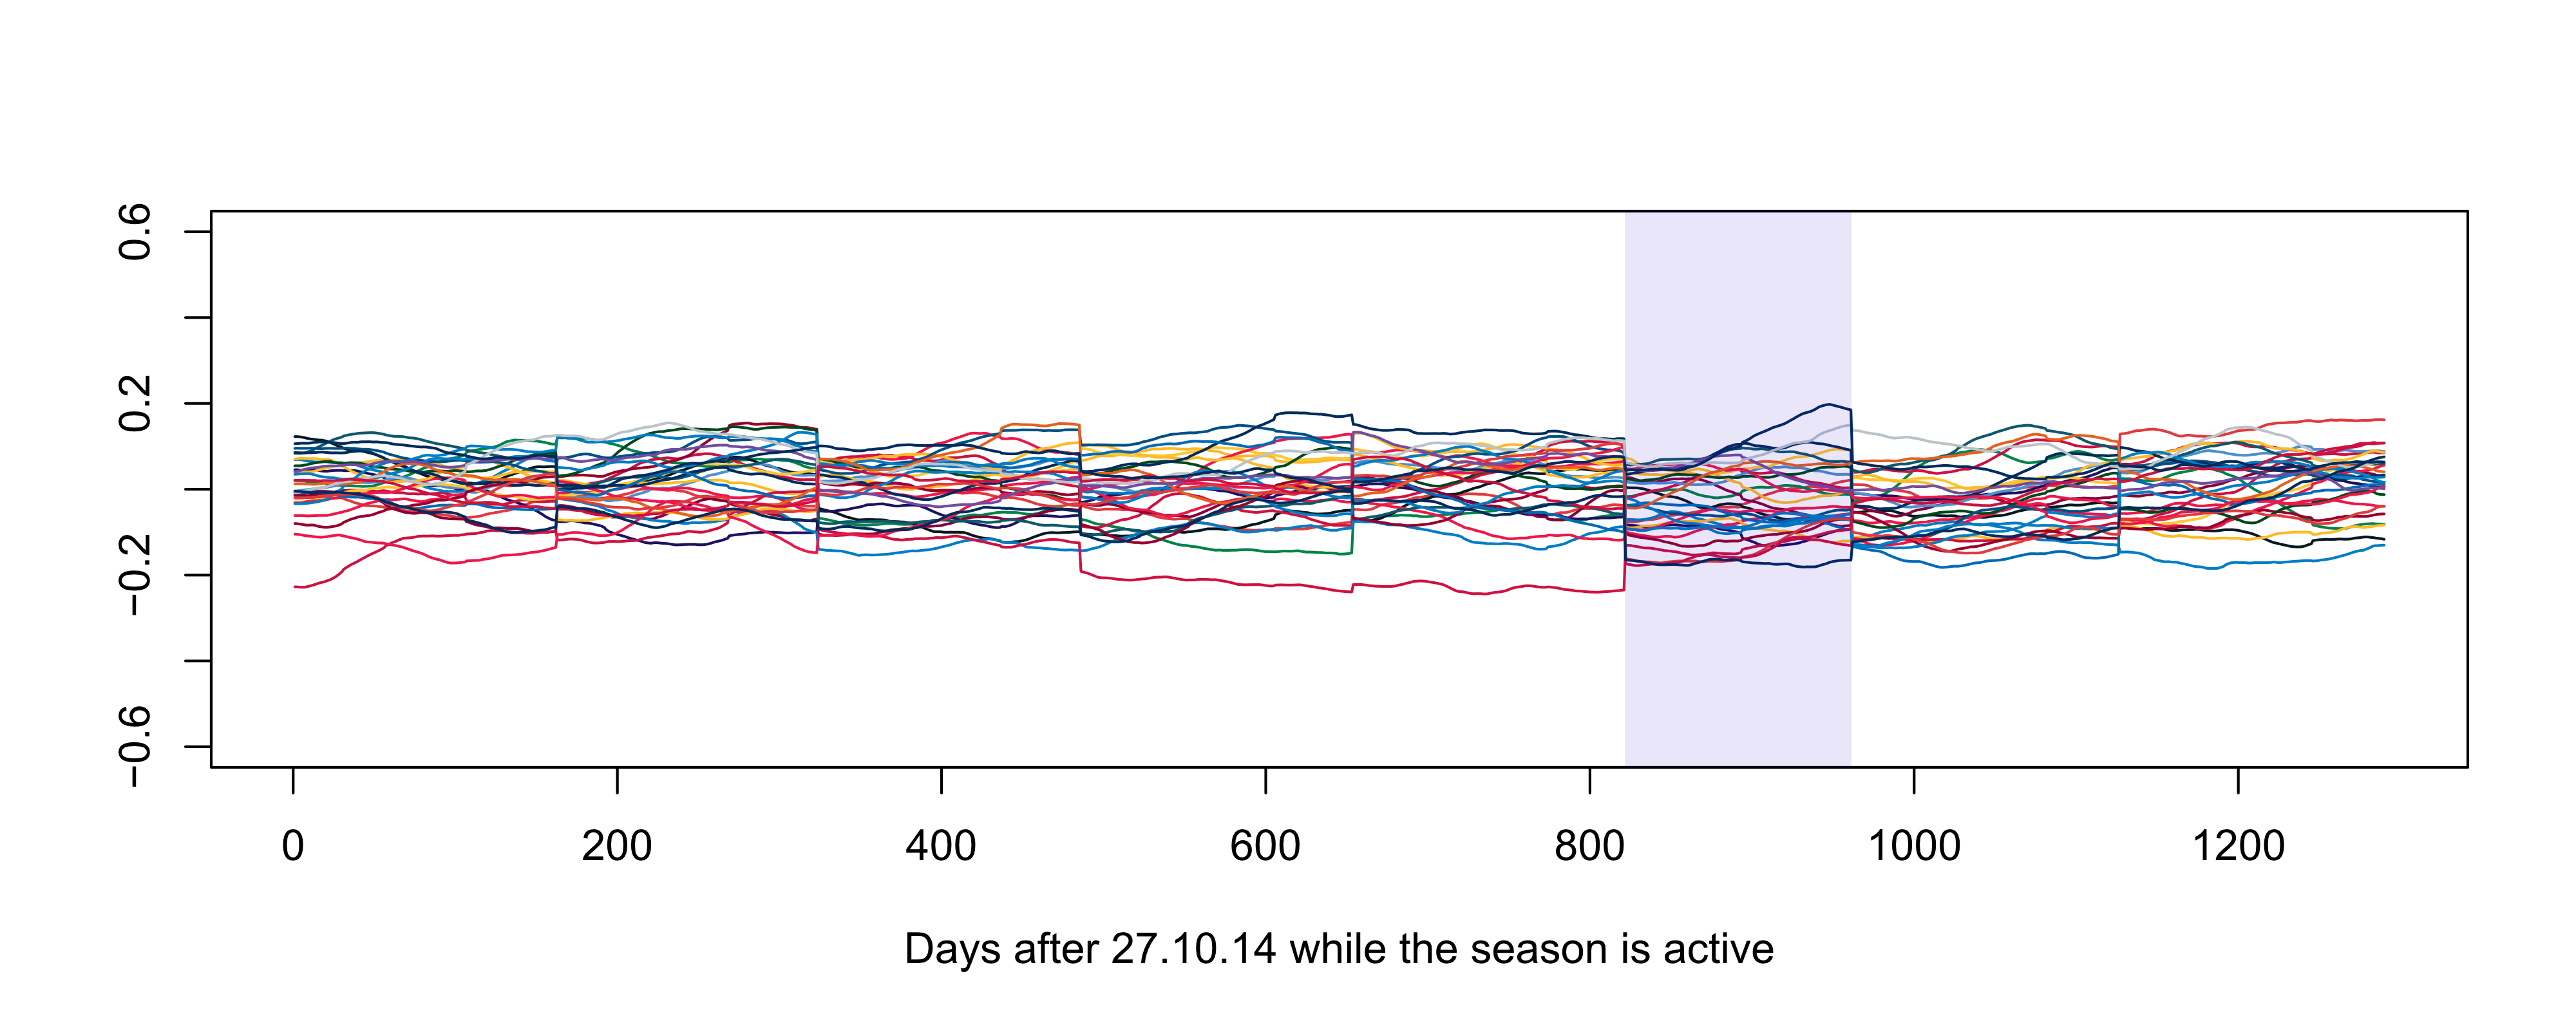
\includegraphics[width=1\textwidth]{Figures/OU2.png}
    \caption[OU2]{Strength of attacking type 2 using the OU model where the highlighted area is the covid season}
    \label{fig:OU2}
\end{figure}

\begin{figure}[H]
    \centering
    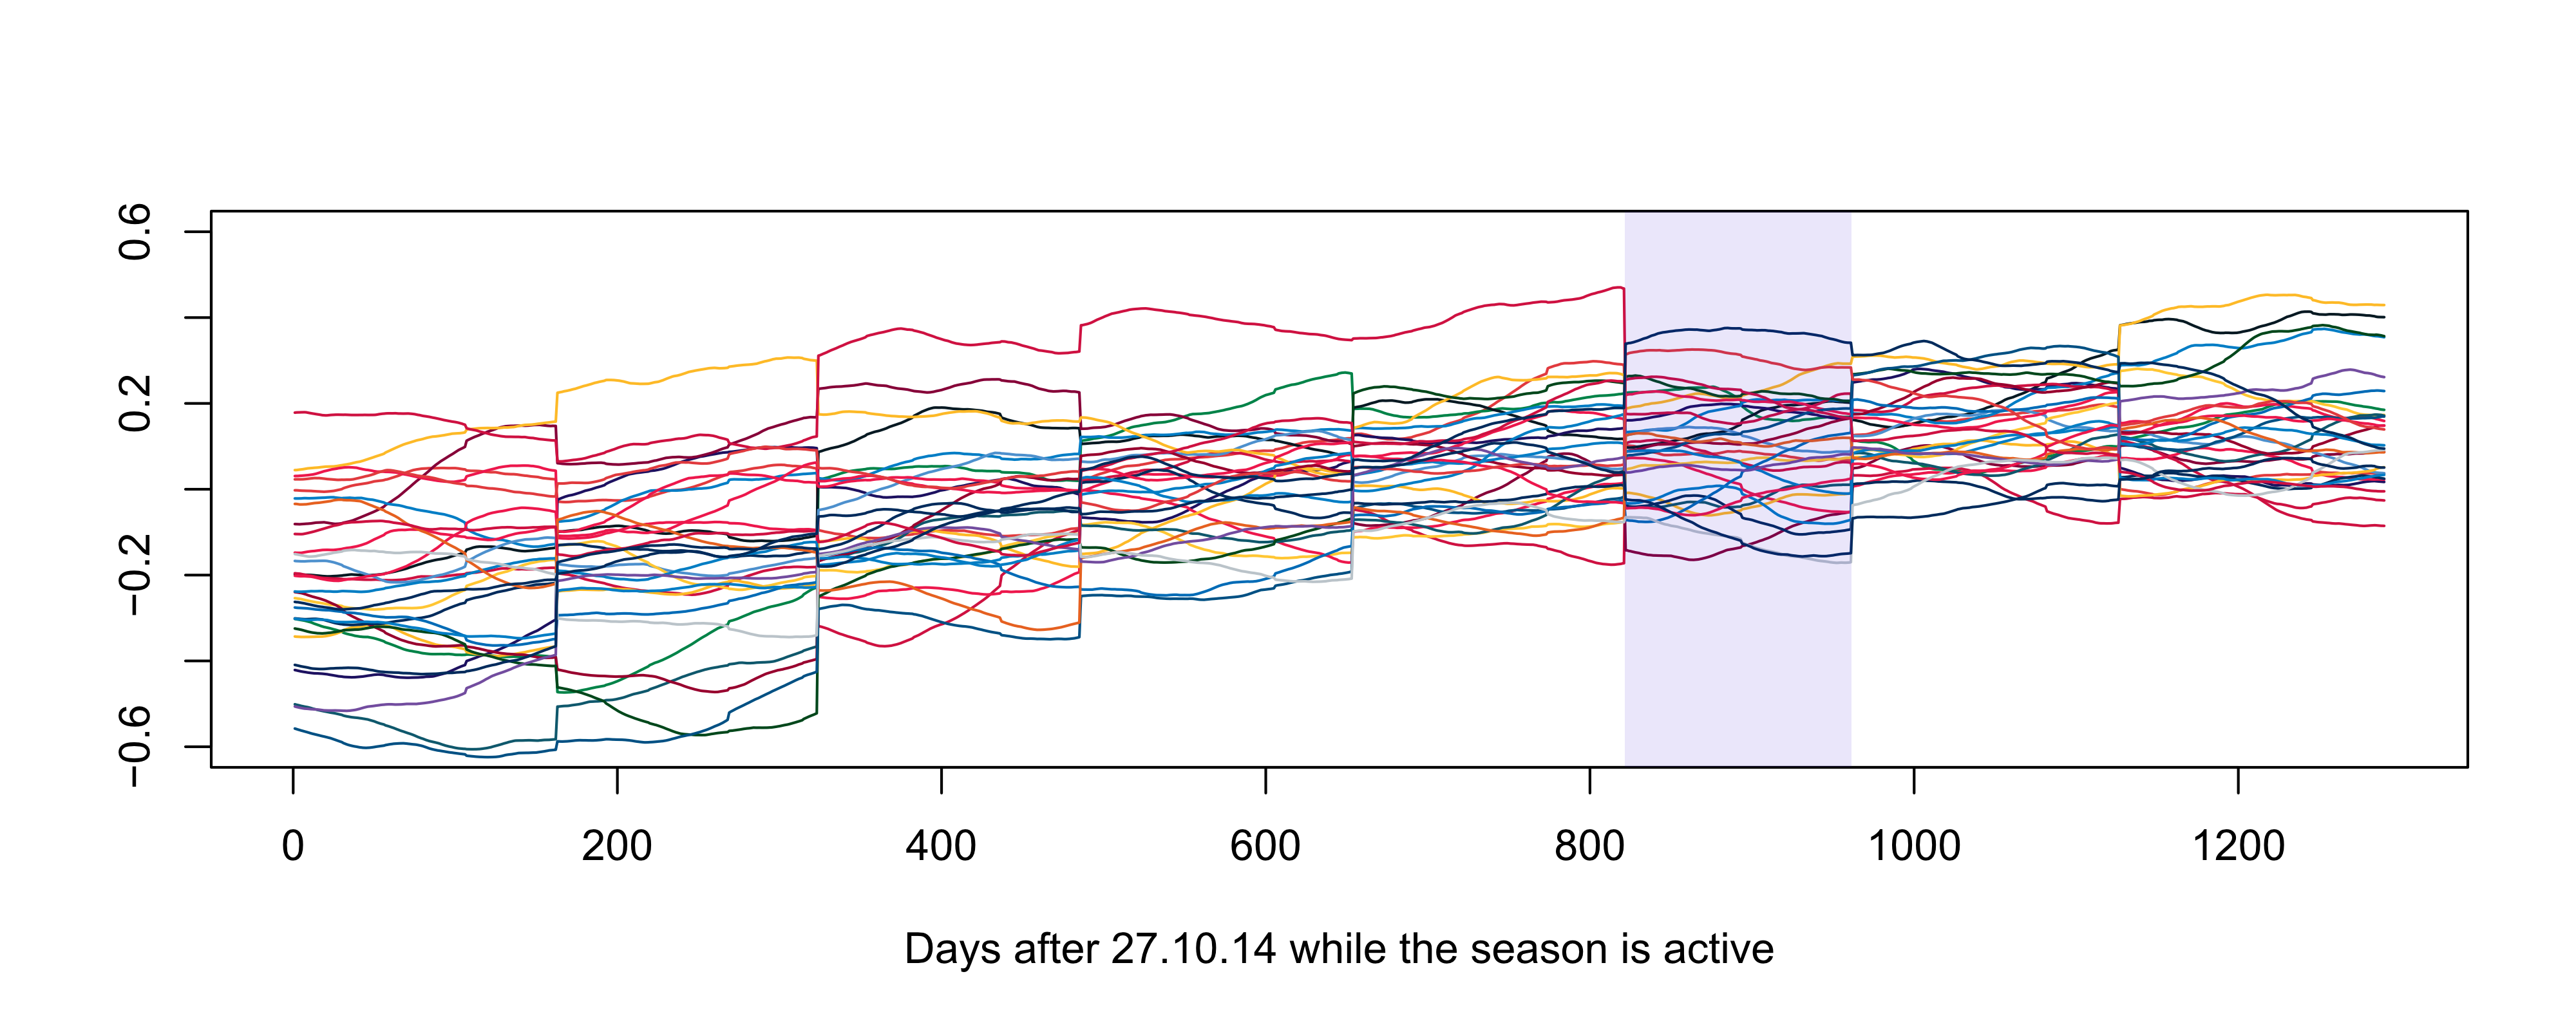
\includegraphics[width=1\textwidth]{Figures/OU3.png}
    \caption[OU3]{Strength of attacking type 3 using the OU model where the highlighted area is the covid season}
    \label{fig:OU3}
\end{figure}

\begin{figure}[H]
    \centering
    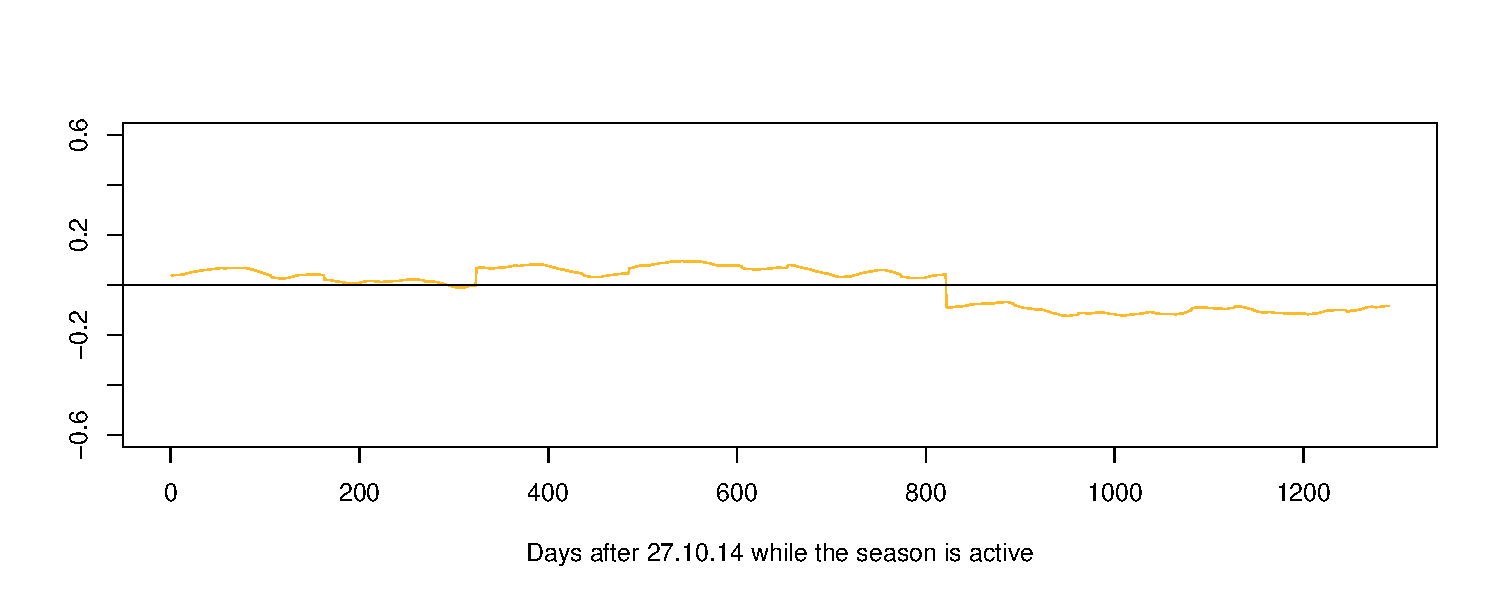
\includegraphics[width=.8\textwidth]{Figures/GSWOU2.pdf}
    \caption[GSW2OU]{GSW Attack strength type 2}
    \label{fig:GSW_2_OU}
\end{figure}

\begin{figure}[H]
    \centering
    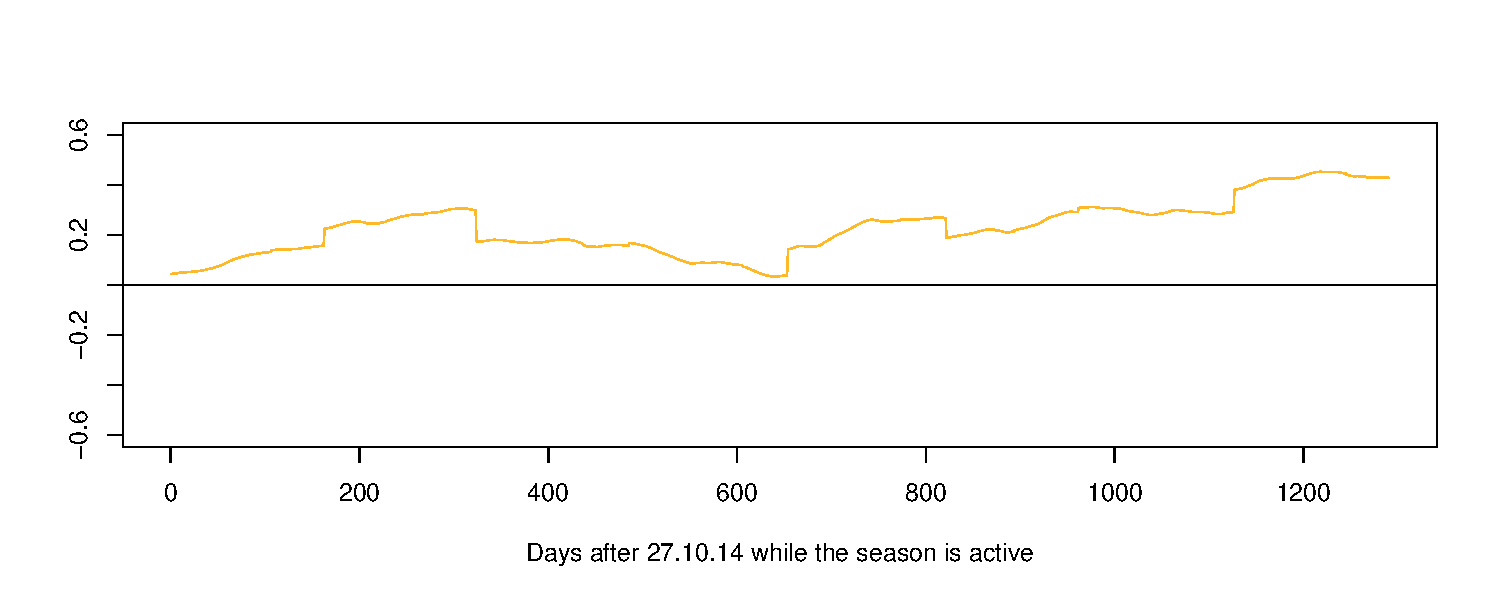
\includegraphics[width=.8\textwidth]{Figures/GSWOU3.pdf}
    \caption[GSW3OU]{GSW Attack strength type 3}
    \label{fig:GSW_3_OU}
\end{figure}

\begin{figure}[H]
    \centering
    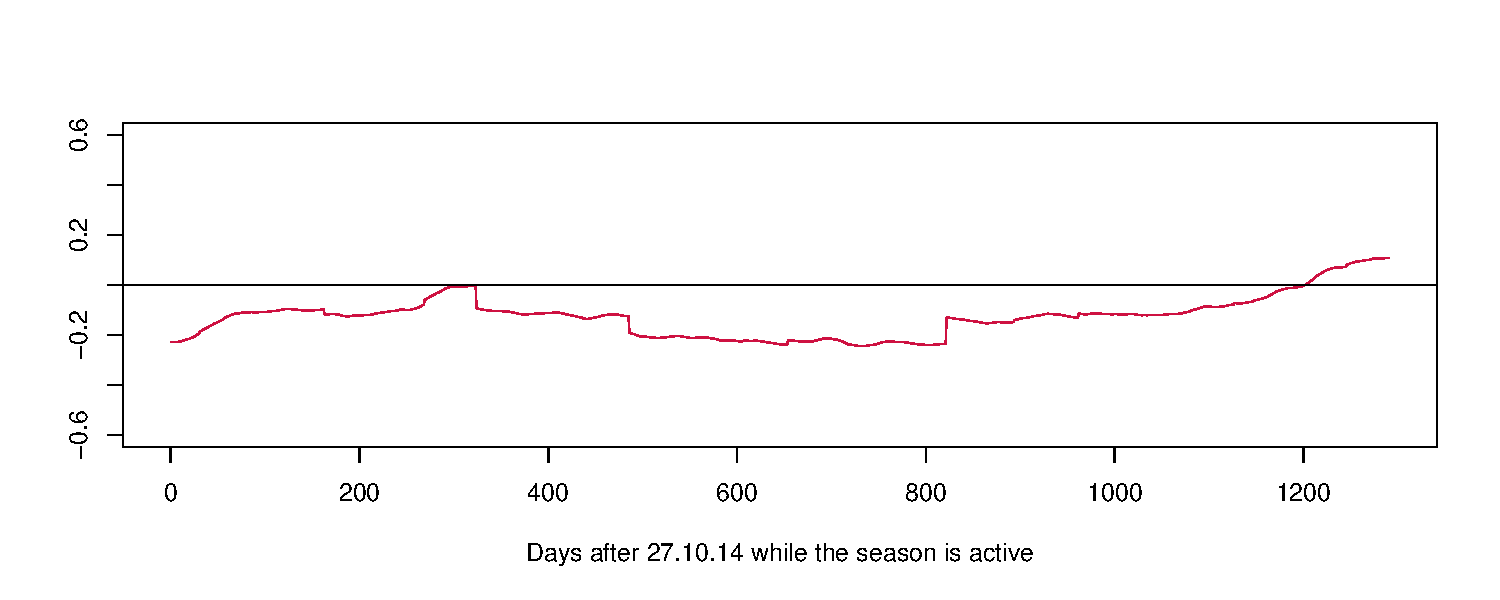
\includegraphics[width=.8\textwidth]{Figures/HOUOU2.pdf}
    \caption[HOU2OU]{HOU Attack strength type 2}
    \label{fig:HOU_2_OU}
\end{figure}

\begin{figure}[H]
    \centering
    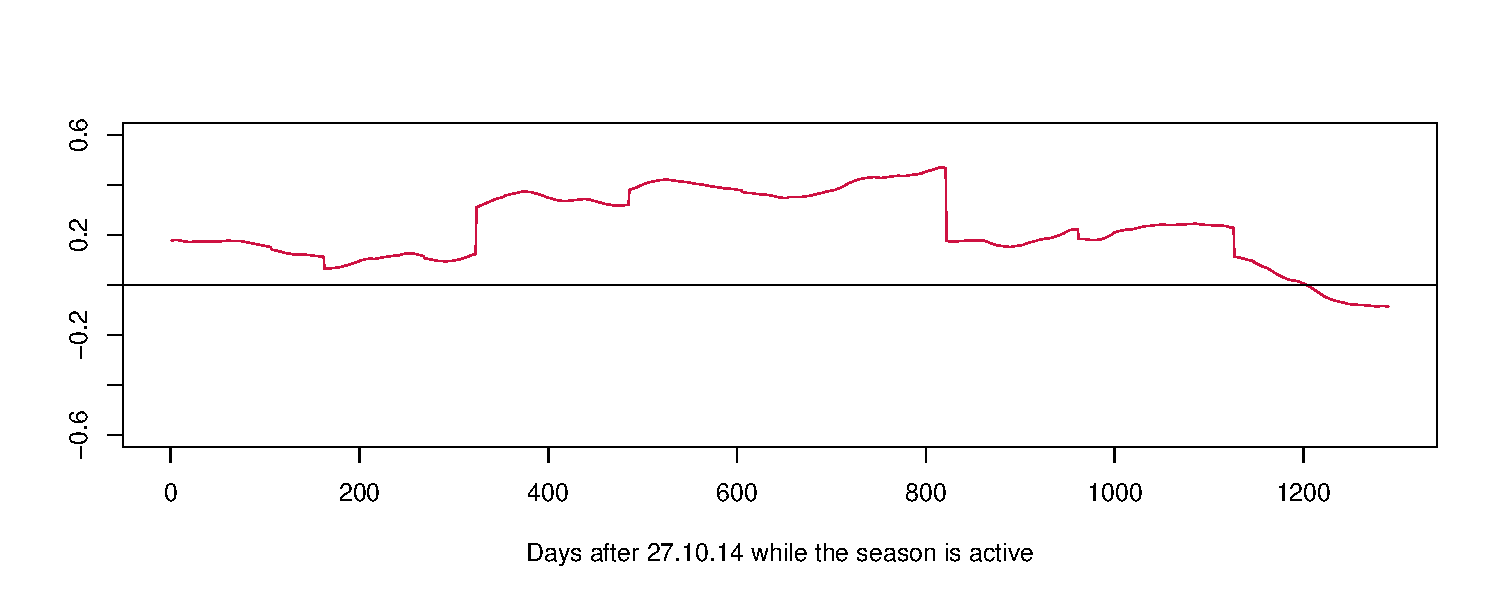
\includegraphics[width=.8\textwidth]{Figures/HOUOU3.pdf}
    \caption[HOU3OU]{HOU Attack strength type 3}
    \label{fig:HOU_3_OU}
\end{figure}

\newpage

\section{Future work}  \label{future}

\noindent The variance of the number of fouls committed in a match is difficult to account for, because it is random, but in close matches there are an overabundance of fouls committed in an attempt to catch up to the opponent, which is closer looked at in \cite{poissonNBA}. To show that there is overdispersion for this in the data, I will first assume that the number of fouls committed, $X$ in a match is Poisson distributed with rate $\lambda$, I will also assume that the number of scores, $Y$, conditional on the number of fouls is binomially distributed with parameters $2X$ and $p$, where we have an average of 2 attempts per foul. I.e.,

\begin{equation}
    X \sim Poisson(\lambda),
\end{equation}

\begin{equation}
    Y|X=x \sim Bin(2X,p).
\end{equation}

\noindent For finding the marginal expectation and variance of $Y$, I will use the law of total expectation and law of total variance.

\begin{equation}
\begin{aligned}
    E[Y] &= E[E[Y|X]] \\
        &= E[2Xp] \\
        &= 2\lambda p
\end{aligned}
\end{equation}

\begin{equation}
\begin{aligned}
    Var[Y] &= E[Var[Y|X]] + Var[E[Y|X]] \\
        &= E[2Xp(1-p)] + Var[2Xp] \\
        &= 2\lambda p(1-p) + 4p^2\lambda \\
        &= E[y](1-p + 2p) \\
        &= E[y](1 + p) \\
\end{aligned}
\end{equation}

\noindent Since $(1 + p)$ is larger than one, this underlying data-generating process would generate overdispersion in the data.
